\documentclass[
  unicode,a4paper,10pt,
  % aspectratio=169,
  xcolor = {dvipsnames,svgnames},
  hyperref ={colorlinks=true,citecolor=Navy,linkcolor=NavyBlue,urlcolor=purple},
  ja=standard,lualatex
]{beamer}
\renewcommand{\baselinestretch}{1.4}

% ---fonts---
\usefonttheme{serif}
\mathversion{bold}
\usepackage{luatexja-fontspec}
\setmainfont{TeX Gyre Termes}
\setmainjfont{Noto Sans JP}
\setmathrm{Latin Modern Roman}
% \setmainjfont{IPAexGothic}

% ---refer `texdoc xcolor' at the command line---

% ---Display \subsubsection at the Index
% \setcounter{tocdepth}{3}

% ---Setting about the geometry of the document----
% \usepackage{a4wide}
% \pagestyle{empty}

% ---Physics and Math Packages---
\usepackage{amssymb,amsfonts,amsthm,mathtools}
\usepackage{physics,braket}
\usepackage{bm}

% ---underline---
\usepackage[normalem]{ulem}

% ---cancel---
\usepackage{cancel}

% --- surround the texts or equations
\usepackage{fancybox,ascmac}

% ---settings of theorem environment---
% \usepackage{amsthm}
% \theoremstyle{definition}

% ---settings of proof environment---
% \renewcommand{\proofname}{\textbf{証明}}
% \renewcommand{\qedsymbol}{$\blacksquare$}

% ---Insert the figure (If insert the `draft' at the option, the process becomes faster.)---
\usepackage{graphicx}
% \usepackage{subcaption}

% ----Add a link to a text---
\usepackage{url,hyperref}
\usepackage{xcolor}

% ---Tikz---
\usepackage{tikz,pgf,pgfplots,circuitikz}
\pgfplotsset{compat=1.15}
\usetikzlibrary{intersections,arrows.meta,angles,calc,3d,decorations.pathmorphing,positioning}

% ---Add the section number to the equation, figure, and table number---
\makeatletter
   \renewcommand{\theequation}{\thesection.\arabic{equation}}
   \@addtoreset{equation}{section}
   
   \renewcommand{\thefigure}{\thesection.\arabic{figure}}
   \@addtoreset{figure}{section}
   
   \renewcommand{\thetable}{\thesection.\arabic{table}}
   \@addtoreset{table}{section}
\makeatother

% ---enumerate---
% \renewcommand{\labelenumi}{$\arabic{enumi}.$}
% \renewcommand{\labelenumii}{$(\arabic{enumii})$}

% ---beamer settings---
\usefonttheme{professionalfonts}
\usecolortheme{seahorse}
\setbeamercolor{structure}{fg=white}
\setbeamercolor{local structure}{fg=red}
\setbeamertemplate{itemize item}[ball]
\setbeamertemplate{enumerate item}[circle]
\setbeamercolor{bibliography entry author}{fg=black}
\setbeamercolor{bibliography item}{fg=black}
\setbeamercolor{alerted text}{fg=RoyalBlue}
\setbeamertemplate{frametitle continuation}{}
\setbeamertemplate{footline}[frame number]
\setbeamertemplate{navigation symbols}{} 
\setbeamersize{text margin left=10pt, text margin right=10pt}

% ---tcolorbox---
\usepackage{tcolorbox}
\tcbuselibrary{theorems}
\tcbuselibrary{raster}
\tcbuselibrary{skins}
\newtcolorbox{bluebox}[2][]{enhanced,
colframe=RoyalBlue!40!white,
colback=RoyalBlue!10!white,
coltitle=black,
drop fuzzy shadow, title={#2}
,#1}
\newtcolorbox{redbox}[2][]{enhanced,
colframe=DarkRed!40!white,
colback=DarkRed!10!white,
coltitle=black,
drop fuzzy shadow, title={#2}
,#1}

% ---Ignore the Warnings---
\usepackage{silence}
\WarningFilter{latexfont}{Some font shapes}
\WarningFilter{latexfont}{Font shape}
\ExplSyntaxOn
\msg_redirect_name:nnn{hooks}{generic-deprecated}{none}
\ExplSyntaxOff

% \usepackage{newtxmath}

% ---citation---
\usepackage{usebib}
\newbibfield{author} 
\newbibfield{year} 
\newbibfield{journal} 
\newbibfield{doi} 
\bibinput{ref}

\makeatletter
\newcommand*{\journal}{\begingroup\@makeother\#\@mylink}
\newcommand*{\@mylink}[1]{\href{http://dx.doi.org/\usebibentry{#1}{doi}}{\usebibentry{#1}{journal}}\endgroup} 
\makeatother

\newcommand*{\citefone}[2]{
  \begin{tikzpicture}[remember picture, overlay]
    \node[anchor=north east, align=left] at ($(current page.north east)-(0,0.0)$){
    {\tiny
      \cite{#1}
      #2,
      \journal{#1}
      (\usebibentry{#1}{year}).
    }
    };
  \end{tikzpicture}
}

\newcommand*{\citeftwo}[4]{
  \begin{tikzpicture}[remember picture, overlay]
    \node[anchor=north east, align=left] at ($(current page.north east)-(0,0.0)$){
    {\tiny
      \cite{#1}
      #2,
      \journal{#1}
      (\usebibentry{#1}{year}).
    }
    \\[-2.4ex]
    {\tiny
      \cite{#3}
      #4,
      \journal{#3}
      (\usebibentry{#3}{year}).
    }
    };
  \end{tikzpicture}
}

\newcommand*{\citefthree}[6]{
  \begin{tikzpicture}[remember picture, overlay]
    \node[anchor=north east, align=left] at ($(current page.north east)-(0,0.0)$){
    {\tiny
      \cite{#1}
      #2,
      \journal{#1}
      (\usebibentry{#1}{year}).
    }
    \\[-2.4ex]
    {\tiny
      \cite{#3}
      #4,
      \journal{#3}
      (\usebibentry{#3}{year}).
    }
    \\[-2.4ex]
    {\tiny
      \cite{#5}
      #6,
      \journal{#5}
      (\usebibentry{#5}{year}).
    }
    };
  \end{tikzpicture}
}

\newcommand*{\citefonev}[3]{
  \begin{tikzpicture}[remember picture, overlay]
    \node[anchor=north east, align=left, text width=#3cm] at ($(current page.north east)-(0,0.0)$){
    {{\fontsize{5pt}{0pt}\selectfont
      \cite{#1}
      #2,
      \journal{#1}
      (\usebibentry{#1}{year}).\par}
    }
    };
  \end{tikzpicture}
}

\newcommand*{\citeftwov}[5]{
  \begin{tikzpicture}[remember picture, overlay]
    \node[anchor=north east, align=left, text width=#5cm] at ($(current page.north east)-(0,0.0)$){
    {{\fontsize{5pt}{0pt}\selectfont
      \cite{#1}
      #2,
      \journal{#1}
      (\usebibentry{#1}{year}).\par}

      {\fontsize{5pt}{0pt}\selectfont
      \cite{#3}
      #4,
      \journal{#3}
      (\usebibentry{#3}{year}).\par}
    }
    };
  \end{tikzpicture}
}

\newcommand*{\citefthreev}[7]{
  \begin{tikzpicture}[remember picture, overlay]
    \node[anchor=north east, align=left, text width=#7cm] at ($(current page.north east)-(0,0.0)$){
    {{\fontsize{5pt}{0pt}\selectfont
    \cite{#1}
    #2,
    \journal{#1}
    (\usebibentry{#1}{year}).\par}

    {\fontsize{5pt}{0pt}\selectfont
    \cite{#3}
    #4,
    \journal{#3}
    (\usebibentry{#3}{year}).\par}

    {\fontsize{5pt}{0pt}\selectfont
    \cite{#5}
    #6,
    \journal{#5}
    (\usebibentry{#5}{year}).\par}
    }
    };
  \end{tikzpicture}
}


% ---Title---
\title{
  Spring School 2024
}
\author{
  Abe Lab. \ M1
  \texorpdfstring{\\}{}
  \texorpdfstring{\vspace*{3pt}}{}
  Itsuki Miyane
}
\date{Sunday, April 7th, 2024}


\begin{document}

\begin{frame}

  \setbeamertemplate{blocks}[rounded][shadow=true]
  \setbeamercolor{block body}{bg=blue!10!white, fg=black}

  \begin{block}{}
    \centering
    Spring School 2024 @Izukawana
    \\
    \Large
    Moduli stabilization

    on (for/at/in ?) supersymmetric magnetized D9-brane model
  \end{block}

  \begin{center}
    Abe Lab. \ M1 \\
    Itsuki Miyane

    \vspace*{5pt}

    Sunday, April 7th, 2024
  \end{center}

  \begin{center}
    $^{\ast}$I will speak in Japanese though this slide is written in English.
  \end{center}
\end{frame}

\begin{frame}{Topics}
  \begin{itemize}
    \item
          Reviewing the senior thesis
    \item
          Reporting progress and difficulties I met
  \end{itemize}
\end{frame}


\section{Introduction}

\begin{frame}
  \huge \secname
\end{frame}

\begin{frame}{Motivation}

  To solve the problems in the Standard Model, \textcolor{Green}{higher dimensional models} were proposed.

  \vspace{10pt}

  \pause

  In general, these theories contain extra fields related to
  \begin{itemize}
    \item
          the size and shape of the compactified extra dimension,
    \item
          hence the metric and the gravity
  \end{itemize}
  in its 4d effective field theory.

  \vspace{10pt}

  \pause

  \setbeamertemplate{blocks}[rounded][shadow=true]
  \setbeamercolor{block body}{bg=LimeGreen!10!white, fg=black}

  \begin{block}{}
    \centering
    \large
    Such a field is called \textcolor{DarkMagenta}{\textbf{moduli fields}}.
  \end{block}

\end{frame}


\begin{frame}{Moduli stabilization}

  The metrics in 10-dimensional spacetime are dynamical fields:
  \begin{align}
    \dd s^{10}
     & =
    \textcolor{DarkBlue}{G_{MN}(X)}\dd X^{M}\dd X^{N}
    \nonumber
    \\
     & =
    \textcolor{DarkBlue}{g_{\mu\nu}(x,y)}\dd x^{\mu}\dd x^{\nu}
    +
    \textcolor{DarkBlue}{g_{mn}(x,y)}\dd y^{m}\dd y^{n}
    \nonumber
  \end{align}

  Thus, its vacuum expectation value (VEV) should be determined \textbf{\textcolor{Goldenrod}{by its dynamics}}.

  \pause

  \uline{How?}

  \begin{columns}[t]
    \begin{column}{0.4\textwidth}
      What we have to do is just
      \begin{itemize}
        \item
              Write down the potential \\
              for moduli (\uline{e.g.}\ \  $g_{mn}$)
        \item
              Compute the minimum and \\
              identify the value $\ev*{g_{mn}}$
      \end{itemize}
    \end{column}
    \begin{column}{0.4\textwidth}
      \vspace*{-20pt}
      \begin{center}
        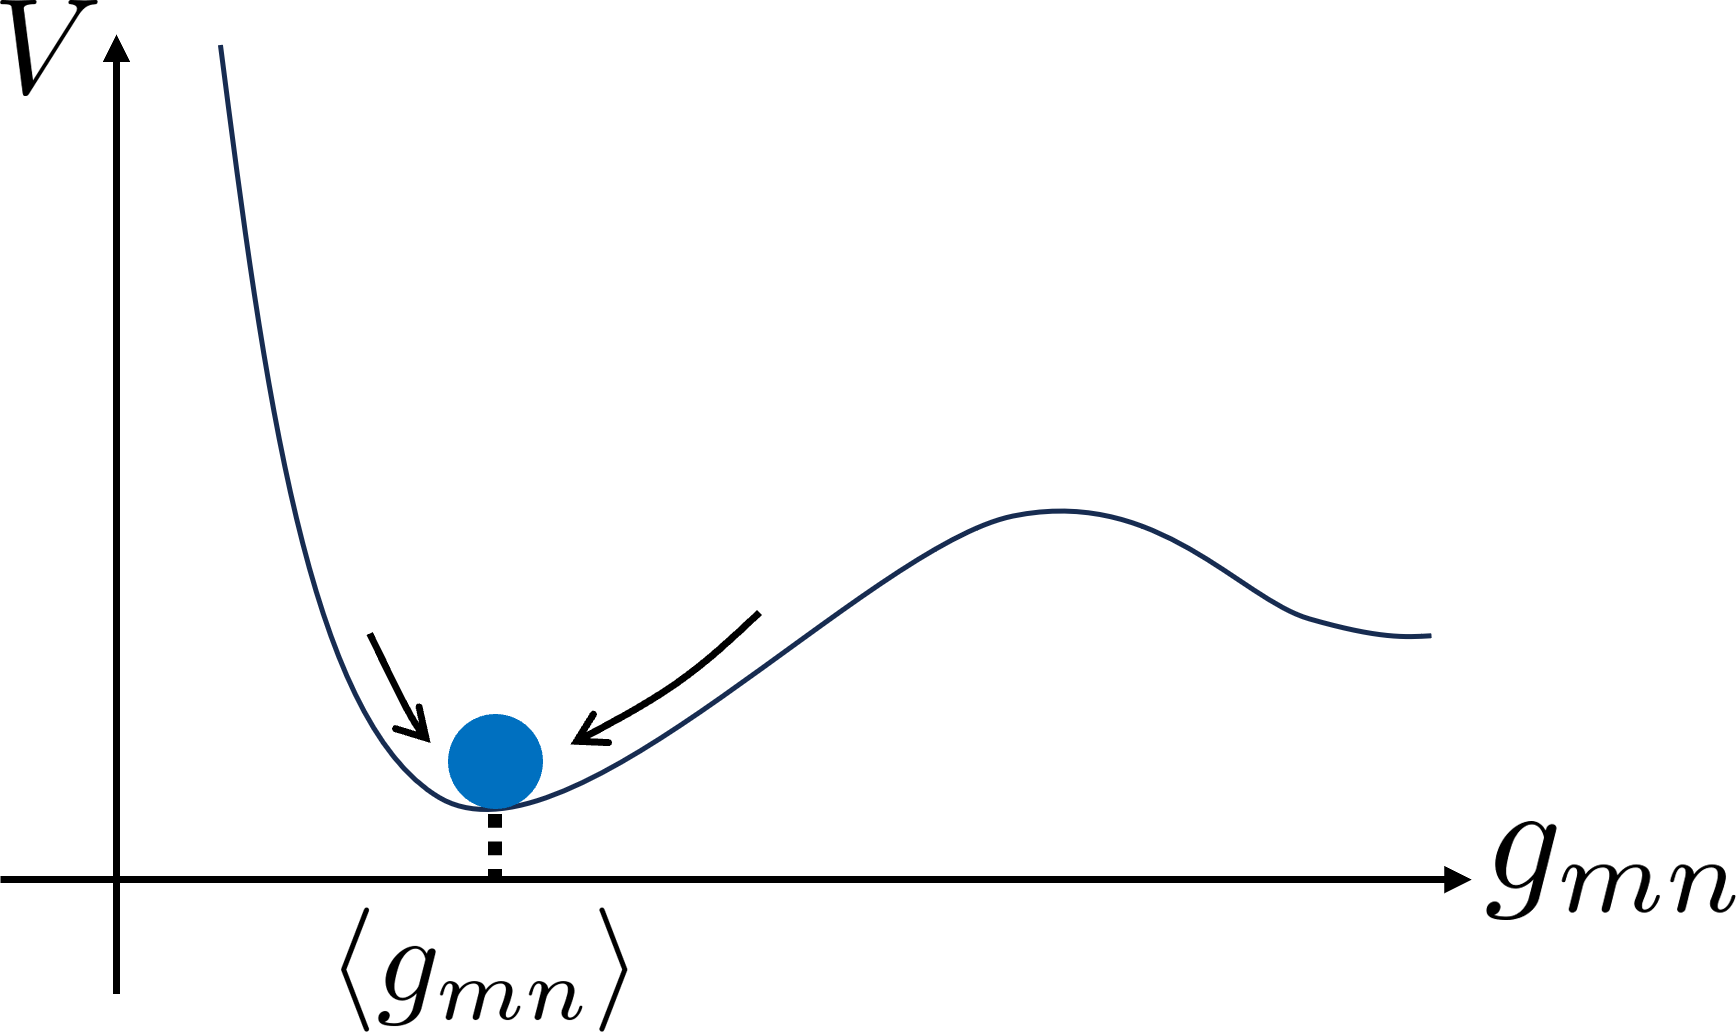
\includegraphics[width=1.0\textwidth]{fig/vev_idea.png}
      \end{center}
    \end{column}
  \end{columns}

  \vspace{10pt}

  These procedures are called \textbf{\textcolor{red}{moduli stabilization}}.

\end{frame}


\begin{frame}{Purpose of our study}
  \citeftwo{Abe:2012ya}{H. Abe, T. Kobayashi, H. Ohki, and K. Sumita}{Abe:2017gye}{H. Abe, T. Kobayashi, K. Sumita, and S. Uemura}
  On the other hand, it is known that \textbf{\textcolor{DarkOrange}{magnetized torus model}}.
  \begin{itemize}
    \item
          \textcolor{DarkOrange}{This model} realize the generation structure of the Standard Model \cite{Abe:2012ya,Abe:2017gye}.

          \pause

    \item
          But the VEVs of the \textcolor{DarkMagenta}{moduli} are not determined dynamically.
  \end{itemize}

  \vspace*{15pt}

  \pause

  \setbeamertemplate{blocks}[rounded][shadow=true]
  \setbeamercolor{block body}{bg=red!10!white, fg=black}

  \begin{block}{}
    \centering
    \large
    We will discuss the \textcolor{red}{moduli stabilization} on \textcolor{DarkOrange}{magnetized torus model}.
  \end{block}

\end{frame}


\section{Magnetized torus model}

\begin{frame}
  \huge \secname
\end{frame}

\begin{frame}{Torus compactification and Magnetic flux}
  \citefone{Abe:2012ya}{H. Abe, T. Kobayashi, H. Ohki, and K. Sumita}
  \uline{Torus compactification}
  \begin{itemize}
    \item
          Compactifying 6d extra dimensions for three tori $(T^2)^3$.
          \\
          \vspace*{5pt}
          \hspace*{2.8cm}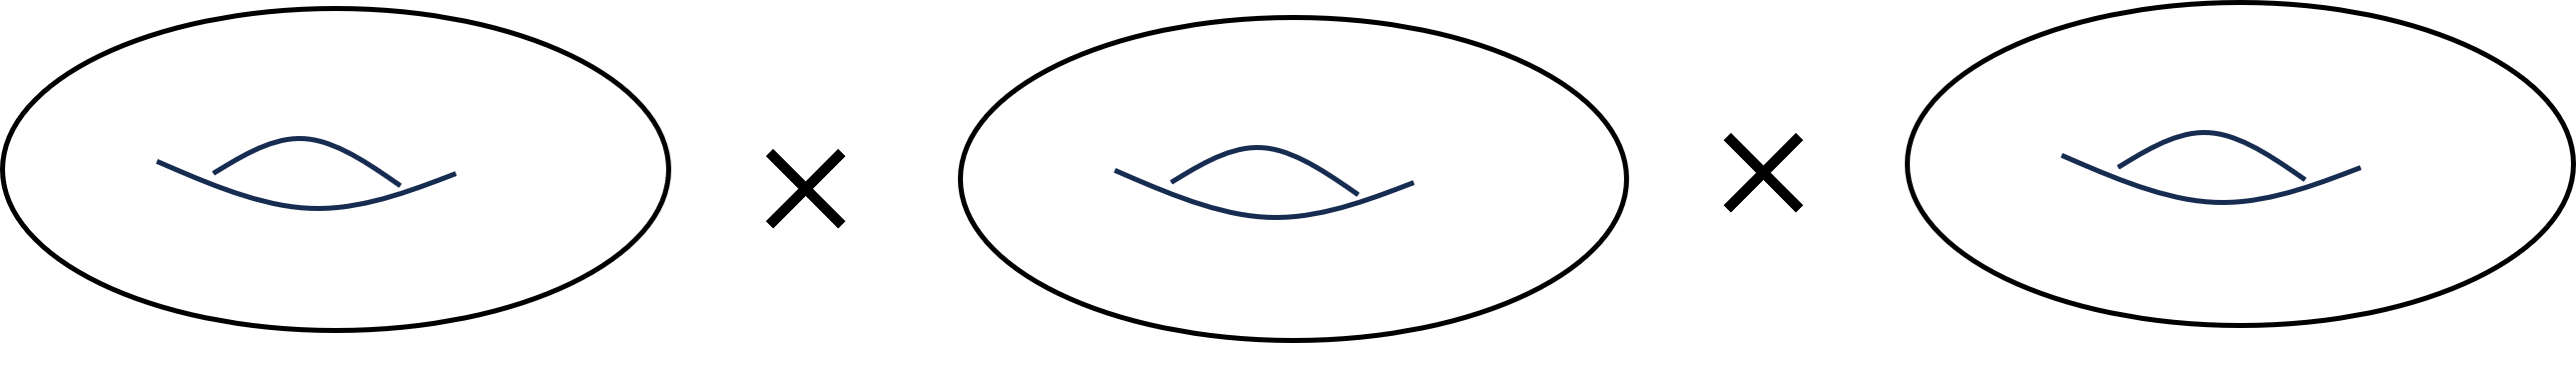
\includegraphics[width=0.4\textwidth]{fig/tori.png}
          \\
          \hspace*{3.0cm}
          $\textcolor{DarkMagenta}{\mathcal{A}^{(1)}}$
          \hspace*{1.0cm}
          $\textcolor{DarkMagenta}{\mathcal{A}^{(2)}}$
          \hspace*{1.0cm}
          $\textcolor{DarkMagenta}{\mathcal{A}^{(3)}}$
          \hspace*{0.5cm}
          : area of the $i$-th torus
    \item
          $\textcolor{DarkMagenta}{\mathcal{A}^{(i)}(x)}$ are also \textcolor{DarkMagenta}{moduli} since it is related to the metric.
  \end{itemize}

  \vspace*{15pt}

  \pause

  \begin{columns}[t]
    \begin{column}{0.5\textwidth}
      \uline{\textcolor{DarkOrange}{Magnetic flux}}
      \begin{itemize}
        \item
              Assigning the magnetic flux\\
              \qquad  $\textcolor{DarkOrange}{M_{a}^{(i)}}\ (a=1,2)$
              \\
              for two gauge fields on each tori.
      \end{itemize}
    \end{column}
    \begin{column}{0.48\textwidth}
      \vspace*{-15pt}
      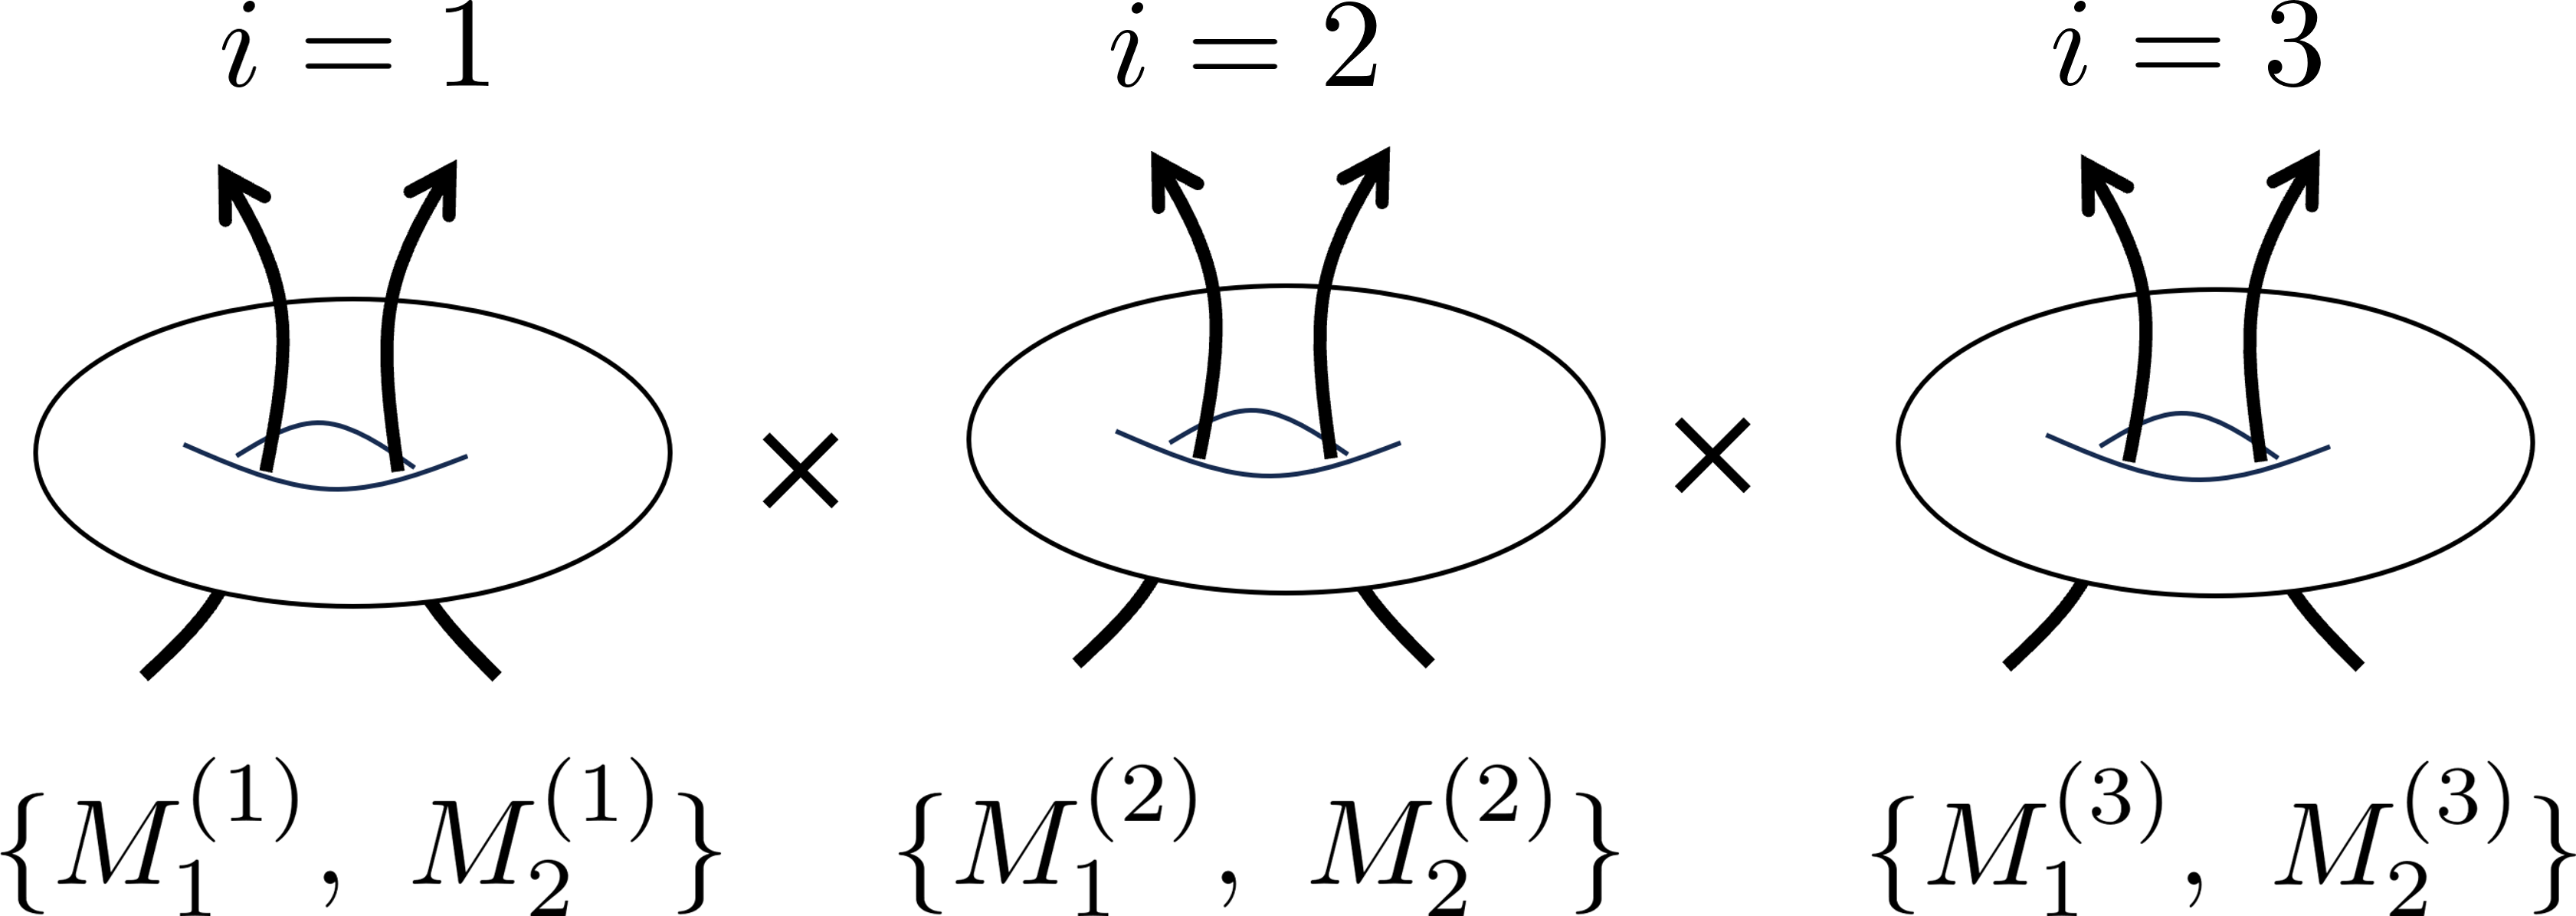
\includegraphics[width=1.0\textwidth]{fig/tori_fluxed.png}
    \end{column}
  \end{columns}

\end{frame}


\begin{frame}{Finding the VEVs by fluxes}
  \citefone{Abe:2012ya}{H. Abe, T. Kobayashi, H. Ohki, and K. Sumita}
  By \textcolor{DarkOrange}{magnetic fluxes} in an extra dimension, \textcolor{DarkMagenta}{moduli $\mathcal{A}^{(i)}(x)$} obtain its potential \textcolor{DarkOrange}{$V^{(D)}$}.

  \vspace{-20pt}

  \begin{center}
    \huge $\downarrow$
  \end{center}

  \vspace{-10pt}

  Finding minima and determining the VEVs of $\ev*{\mathcal{A}^{i}}$.

  \pause

  \vspace{10pt}

  \uline{Potential by \textcolor{DarkOrange}{magnetic fluxes}}\qquad
  $
    F^{MN}F_{MN}
    =
    F^{\mu\nu}F_{\mu\nu}
    +
    \uwave{F^{mn}F_{mn}}
    +
    \cdots
  $
  \\
  \hspace*{9cm}{\Large $\downarrow$}
  \begin{equation}
    \textcolor{DarkOrange}{V^{(D)}}
    =
    \pi^2
    \prod_{i}\mathcal{A}^{i}
    \times
    \left\{
    \uline{
      \left(
      \sum_{i}\frac{M_{1}^{(i)}}{\mathcal{A}^{(i)}}
      \right)^2
    }
    +
    \uline{
      \left(
      \sum_{i}\frac{M_{2}^{(i)}}{\mathcal{A}^{(i)}}
      \right)^2
    }
    \right\}
    \nonumber
  \end{equation}

  \pause

  \begin{center}
    $\longrightarrow$\hspace*{10pt}
    \tikz[baseline=(x.base)]{
      \node(x)[rectangle, fill=DarkRed!10, rounded corners]{
        \
        $
          \displaystyle
          \frac{M_{a}^{(1)}}{\ev*{\mathcal{A}^{(1)}}}
          +
          \frac{M_{a}^{(2)}}{\ev*{\mathcal{A}^{(2)}}}
          +
          \frac{M_{a}^{(3)}}{\ev*{\mathcal{A}^{(3)}}}
          =
          0
          \quad
          \text{for}
          \
          a=1,2$\ };
    }
  \end{center}

\end{frame}


\begin{frame}{Finding the VEVs by fluxes}

  \uline{Relation of the VEVs $\ev*{\mathcal{A}^{(1)}},\ev*{\mathcal{A}^{(2)}},\ev*{\mathcal{A}^{(3)}}$}

  \begin{center}
    \tikz[baseline=(x.base)]{
      \node(x)[rectangle, fill=DarkRed!10, rounded corners]{
        \
        $
          \displaystyle
          \frac{M_{a}^{(1)}}{\ev*{\mathcal{A}^{(1)}}}
          +
          \frac{M_{a}^{(2)}}{\ev*{\mathcal{A}^{(2)}}}
          +
          \frac{M_{a}^{(3)}}{\ev*{\mathcal{A}^{(3)}}}
          =
          0
          \quad
          \text{for}
          \
          a=1,2$\ };
    }
  \end{center}

  \pause

  \vspace*{-20pt}

  \begin{gather}
    \longrightarrow\quad
    M_{a}^{(1)}
    +
    M_{a}^{(2)}
    \frac{\ev*{\mathcal{A}^{(1)}}}{\ev*{\mathcal{A}^{(2)}}}
    +
    M_{a}^{(3)}
    \frac{\ev*{\mathcal{A}^{(1)}}}{\ev*{\mathcal{A}^{(3)}}}
    =
    0
    \nonumber
    \\
    \text{\Large $\downarrow$}
    \nonumber
    \\
    \hspace*{-10pt}
    \frac{\ev*{\mathcal{A}^{(1)}}}{\ev*{\mathcal{A}^{(2)}}}
    =
    \frac{
    M_{1}^{(3)} M_{2}^{(1)}-M_{1}^{(1)} M_{2}^{(3)}
    }{
    M_{1}^{(2)} M_{2}^{(3)}- M_{1}^{(3)} M_{2}^{(2)}
    }
    \ ,\
    \frac{\ev*{\mathcal{A}^{(1)}}}{\ev*{\mathcal{A}^{(3)}}}
    =
    -\frac{
    M_{1}^{(2)} M_{2}^{(1)}-M_{1}^{(1)} M_{2}^{(2)}
    }{
    M_{1}^{(2)} M_{2}^{(3)}-M_{1}^{(3)} M_{2}^{(2)}
    }
    \nonumber
  \end{gather}

  \pause

  \setbeamertemplate{blocks}[rounded][shadow=true]
  \setbeamercolor{block body}{bg=Goldenrod!10!white, fg=black}

  \begin{block}{}
    \centering
    The ratios of the moduli's VEVs are determined by the fluxes potential.
  \end{block}

\end{frame}


\begin{frame}{Summary so far}

  \begin{itemize}
    \item
          We could stabilize the moduli\\
          and obtain the ratio of its VEVs $\textcolor{DarkMagenta}{\ev*{\mathcal{A}^{(1)}}/\ev*{\mathcal{A}^{(2)}}\ \&\ \ev*{\mathcal{A}^{(1)}}/\ev*{\mathcal{A}^{(3)}}}$.
          \pause
    \item
          But the \textcolor{Green}{\textbf{overall factor} $T$} is undetermined.
          \begin{equation}
            \textcolor{Green}{T}
            \propto
            \textcolor{DarkMagenta}{\ev*{\mathcal{A}^{(1)}}} ,
            \textcolor{DarkMagenta}{\ev*{\mathcal{A}^{(2)}}} ,
            \textcolor{DarkMagenta}{\ev*{\mathcal{A}^{(3)}}}
            \nonumber
          \end{equation}
  \end{itemize}

  \vspace*{10pt}

  \pause

  \begin{center}
    Introducing a potential that \textcolor{Goldenrod}{has a different origin} than the magnetic fluxes
    \\
    to stabilize \textcolor{Green}{\textbf{overall factor} $T$}.
  \end{center}

\end{frame}


\section{Determination of the overall factor}

\begin{frame}
  \huge \secname
\end{frame}

\begin{frame}{$F$-term potential}
  \citeftwo{Abe:2006xp}{H. Abe, T. Higaki, T. Kobayashi, and Y. Omura}{Abe:2007yb}{H. Abe, T. Higaki, and T. Kobayashi}
  \uline{Effective potential for \textcolor{Green}{moduli $T$}}
  \begin{itemize}
    \item
          Its effective theory remains supersymmetric.
    \item
          Supersymmetric action is determined\\
          \qquad by \textcolor{RoyalBlue}{\textbf{super potential} $W$} and \textcolor{DarkRed}{\textbf{K\"{a}hler potential} $K$}.
    \item
          We will study the following potential now\cite{Abe:2006xp}:
          \begin{equation}
            \left\{
            \begin{alignedat}{1}
              \textcolor{RoyalBlue}{W}
              &=
              w_{0}-Ae^{-a\textcolor{Green}{T}}+B\textcolor{DarkBlue}{X}
              \\
              \textcolor{DarkRed}{K}
              &=
              -
              3\ln (\textcolor{Green}{T}+\textcolor{Green}{\bar{T}})
              +
              \textcolor{DarkBlue}{|X|^2}
            \end{alignedat}
            \right.
            \nonumber
          \end{equation}
          \begin{center}
            \small
            Introducing a new scalar field $\textcolor{DarkBlue}{X}$
            and
            $w_{0}, A, B, a$ are parameters.
          \end{center}
  \end{itemize}

\end{frame}


\begin{frame}{$F$-term potential}
  \citeftwo{Abe:2006xp}{H. Abe, T. Higaki, T. Kobayashi, and Y. Omura}{Abe:2007yb}{H. Abe, T. Higaki, and T. Kobayashi}
  $^{\ast}$We set the Planck constant as $M_{\text{Pl}}\ (\sim 2.4\times 10^{18}\ \text{GeV})=1$.

  \begin{columns}[t]
    \begin{column}{0.6\textwidth}
      \uline{Scalar potential}
      \vspace*{-5pt}
      \begin{gather}
        V^{(F)}
        =
        e^{K}(K^{I\bar{J}}(D_{I}W)(D_{\bar{J}}\bar{W})-3|W|^2)
        \nonumber
        \\
        \left\{
        \begin{alignedat}{1}
          D_{I}W
          &\equiv
          \partial_{I}W+K_{I}W
          \\
          K^{I\bar{J}}
          &\text{: inverse matrix of $K_{I\bar{J}}$}
        \end{alignedat}
        \right.
        \quad
        (I=X,T)
        \nonumber
      \end{gather}
    \end{column}
    \begin{column}{0.38\textwidth}
      \vspace*{-5pt}
      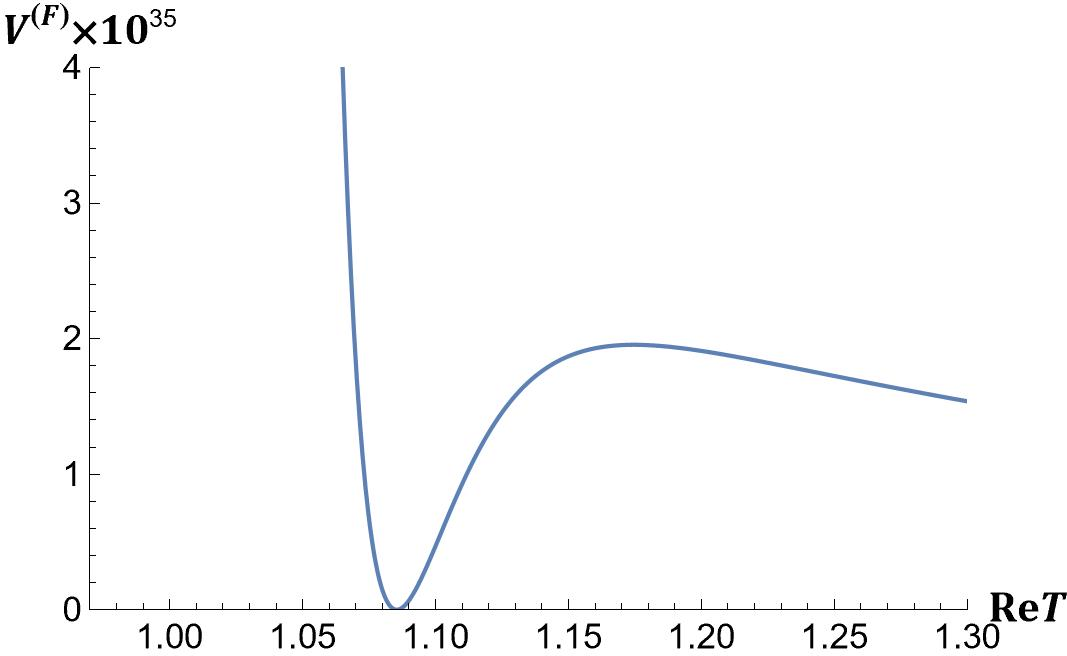
\includegraphics[width=1.0\textwidth]{fig/result.jpg}
    \end{column}
  \end{columns}

  \vspace*{10pt}

  \uline{Parameters}\\
  \begin{center}
    $
      w_{0}
      \sim
      2.17
      \times
      10^{-18}
      \ ,\
      a=4\pi^2
      \ ,\
      A=1
      \ ,\
      B=e^{-4\pi^2}
    $
    \\
    \textbf{and} $\ev*{X}=\sqrt{3}-1$
  \end{center}

  \begin{center}
    $\rightarrow \ev*{T}\sim 1.085$
  \end{center}

\end{frame}

\section{Progresses}

\begin{frame}{Report progresses}

  In my senior thesis, we
  \begin{itemize}
    \item
          fix the value of the \textcolor{DarkOrange}{fluxes $M_{a}^{(i)}$}
    \item
          and compute \textcolor{DarkMagenta}{the area of the tori $\ev*{\mathcal{A}^{(i)}}\ (i=1,2,3)$}.
  \end{itemize}

  \pause
  \citefone{Abe:2007yb}{H. Abe, T. Higaki, and T. Kobayashi}
  During this vacation, I mainly studied the $F$-term potential more general form:
  \begin{equation}
    \left\{
    \begin{alignedat}{1}
      \textcolor{RoyalBlue}{W}
      &=
      w_{0}-Ae^{-a\textcolor{Green}{T}}+B\uwave{e^{-b\textcolor{Green}{T}}}\textcolor{DarkBlue}{X}
      \\
      \textcolor{DarkRed}{K}
      &=
      -
      3\ln (\textcolor{Green}{T}+\textcolor{Green}{\bar{T}})
      +
      \textcolor{DarkBlue}{|X|^2}
      \uwave{-
        \frac{1}{\Lambda^2}
        \textcolor{DarkBlue}{|X|^4}
      }
    \end{alignedat}
    \right.
    \nonumber
  \end{equation}

  \vspace*{-15pt}

  \begin{center}
    \uwave{Wavy factors} are the difference from the previous one.
  \end{center}

\end{frame}


\begin{frame}{Report progresses}

  We can stabilize the moduli $\textcolor{Green}{T}, \textcolor{DarkBlue}{X}$ but $\cdots\cdots$

  \begin{columns}[t]
    \begin{column}{0.5\textwidth}
      \centering
      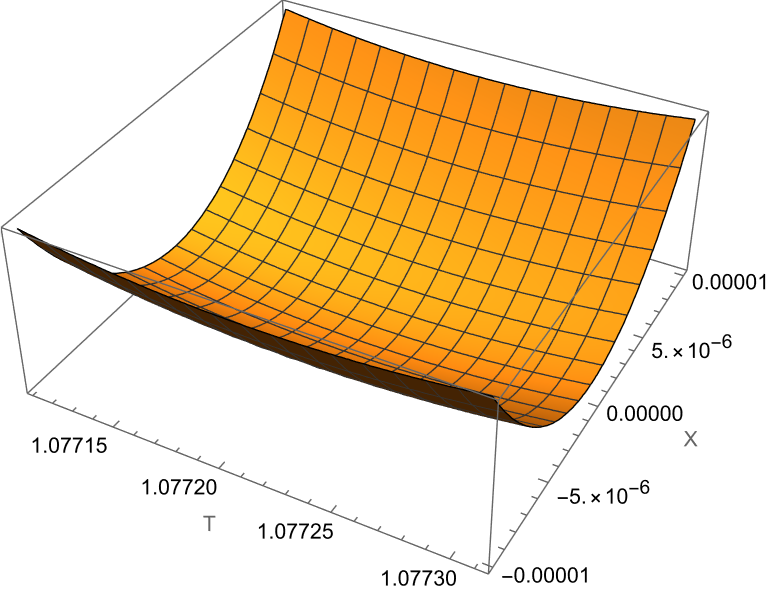
\includegraphics[width=1.0\textwidth]{fig/3dplot.png}
    \end{column}
    \begin{column}{0.5\textwidth}
      \centering
      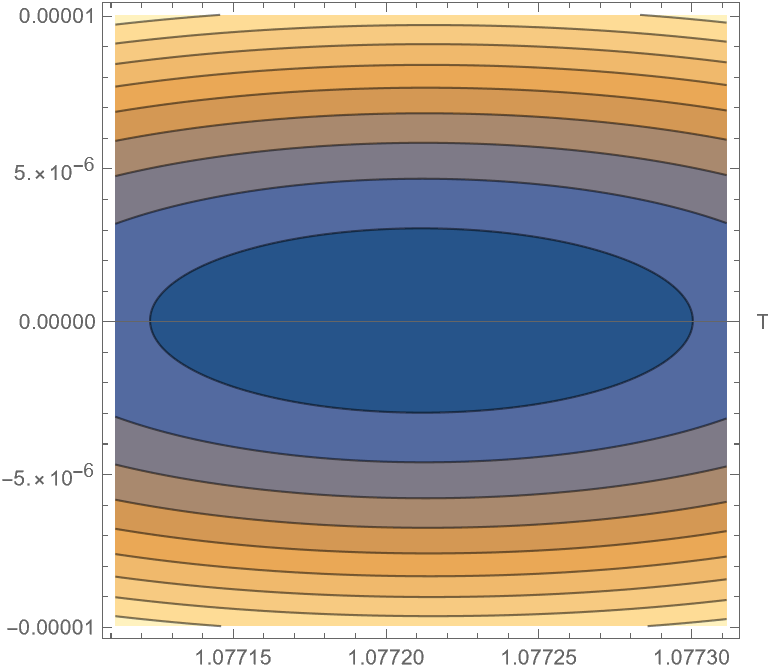
\includegraphics[width=0.8\textwidth]{fig/contourplot.png}
    \end{column}
  \end{columns}

  \uline{Parameters}
  \begin{center}
    $A=B=1, a=b=4\pi^2, w_{0}=10^{-17}, \Lambda=10^{-4}$\\
    $\longrightarrow\quad \textcolor{Green}{\ev*{T}}\sim 1.07,\ \textcolor{DarkBlue}{\ev*{X}}\sim 10^{-8},\ \textcolor{red}{V_{\mathrm{min}}}\sim -10^{-35}$
  \end{center}

\end{frame}


\begin{frame}{Difficulites}

  \begin{itemize}
    \item
          We should tune the parameters $A,B,a,b,w_{0},\Lambda$\\
          to \textbf{uplift the potential minima \textcolor{red}{$V_{\mathrm{min}}$} to the order $+10^{-120}$}.

          \pause

    \item
          But it is difficult (at least for me) since
          \begin{itemize}
            \item
                  we can not find the minimum points analytically
            \item
                  thus what we can do is only\\
                  \qquad \textbf{\textcolor{DarkBlue}{to choose the parameters and find the minimum for each time}}.
          \end{itemize}

          \pause

          \begin{center}
            {\huge \textcolor{DarkBlue}{$\Downarrow$}}
            \\
            I want to find \textcolor{Goldenrod}{more efficient ways to search the set of parameters}.
          \end{center}

          \begin{equation}
            \text{\uline{e.g.}}
            \quad
            \pdv{V}{T}
            =
            \pdv{V}{X}
            =
            0
            \quad
            \&
            \quad
            \pdv{V}{a}
            =
            \pdv{V}{b}
            =
            \pdv{V}{A}
            =
            \pdv{V}{B}
            =
            \pdv{V}{w_{0}}
            =
            0
            \nonumber
          \end{equation}
          \begin{center}
            (I tried it but it seems not to converge the Newtonian method...)
          \end{center}

  \end{itemize}

\end{frame}


\section{Summary}


\begin{frame}{Summary\ \&\ Future Works}

  \uline{Summary}
  \begin{itemize}
    \item
          Discussing moduli stabilization in magnetized torus model
    \item
          Determining the ratio of the moduli by potential $V^{(D)}$ with fluxes
    \item
          Stabilizing the overall moduli $T$ by potential $V^{(F)}$ that has a different origin
  \end{itemize}

  \uline{Future Works}
  \begin{itemize}
    \item
          {[new!]}\ Finding more efficient ways to search the set of parameters.
    \item
          Discussing soft SUSY breaking and mass of supersymmetric particles, etc.
  \end{itemize}

\end{frame}


% --------------------------

\newcounter{Appendix}
\setcounter{Appendix}{\value{framenumber}}
\setcounter{section}{0}
\renewcommand{\thesubsection}{\Alph{subsection}}
\makeatletter
\renewcommand{\theequation}{\thesubsection.\arabic{equation}}
\@addtoreset{equation}{section}

\renewcommand{\thefigure}{\thesubsection.\arabic{figure}}
\@addtoreset{figure}{section}

\renewcommand{\thetable}{\thesubsection.\arabic{table}}
\@addtoreset{table}{section}
\makeatother

% \section{付録}

% \begin{frame}[plain]
%   \frametitle{\ }
%   \huge \secname
% \end{frame}

% \begin{frame}[plain]
%   \frametitle{\thesubsection\ \subsecname}








% \end{frame}

% --------------------------

\nocite{Wess:1992}

\section{Reference}
\begin{frame}[plain,allowframebreaks]{Reference}

  \scriptsize
  \beamertemplatetextbibitems
  \bibliographystyle{ytphys}
  \bibliography{ref}

\end{frame}

\setcounter{framenumber}{\value{Appendix}}
\end{document}
